\documentclass[twoside]{book}

% Packages required by doxygen
\usepackage{calc}
\usepackage{doxygen}
\usepackage{graphicx}
\usepackage[utf8]{inputenc}
\usepackage{makeidx}
\usepackage{multicol}
\usepackage{multirow}
\usepackage{textcomp}
\usepackage[table]{xcolor}

% Font selection
\usepackage[T1]{fontenc}
\usepackage{mathptmx}
\usepackage[scaled=.90]{helvet}
\usepackage{courier}
\usepackage{amssymb}
\usepackage{sectsty}
\renewcommand{\familydefault}{\sfdefault}
\allsectionsfont{%
  \fontseries{bc}\selectfont%
  \color{darkgray}%
}
\renewcommand{\DoxyLabelFont}{%
  \fontseries{bc}\selectfont%
  \color{darkgray}%
}

% Page & text layout
\usepackage{geometry}
\geometry{%
  a4paper,%
  top=2.5cm,%
  bottom=2.5cm,%
  left=2.5cm,%
  right=2.5cm%
}
\tolerance=750
\hfuzz=15pt
\hbadness=750
\setlength{\emergencystretch}{15pt}
\setlength{\parindent}{0cm}
\setlength{\parskip}{0.2cm}
\makeatletter
\renewcommand{\paragraph}{%
  \@startsection{paragraph}{4}{0ex}{-1.0ex}{1.0ex}{%
    \normalfont\normalsize\bfseries\SS@parafont%
  }%
}
\renewcommand{\subparagraph}{%
  \@startsection{subparagraph}{5}{0ex}{-1.0ex}{1.0ex}{%
    \normalfont\normalsize\bfseries\SS@subparafont%
  }%
}
\makeatother

% Headers & footers
\usepackage{fancyhdr}
\pagestyle{fancyplain}
\fancyhead[LE]{\fancyplain{}{\bfseries\thepage}}
\fancyhead[CE]{\fancyplain{}{}}
\fancyhead[RE]{\fancyplain{}{\bfseries\leftmark}}
\fancyhead[LO]{\fancyplain{}{\bfseries\rightmark}}
\fancyhead[CO]{\fancyplain{}{}}
\fancyhead[RO]{\fancyplain{}{\bfseries\thepage}}
\fancyfoot[LE]{\fancyplain{}{}}
\fancyfoot[CE]{\fancyplain{}{}}
\fancyfoot[RE]{\fancyplain{}{\bfseries\scriptsize Generated on Sat Jun 25 2016 10\-:09\-:35 for Effekseer Unity Plugin by Doxygen }}
\fancyfoot[LO]{\fancyplain{}{\bfseries\scriptsize Generated on Sat Jun 25 2016 10\-:09\-:35 for Effekseer Unity Plugin by Doxygen }}
\fancyfoot[CO]{\fancyplain{}{}}
\fancyfoot[RO]{\fancyplain{}{}}
\renewcommand{\footrulewidth}{0.4pt}
\renewcommand{\chaptermark}[1]{%
  \markboth{#1}{}%
}
\renewcommand{\sectionmark}[1]{%
  \markright{\thesection\ #1}%
}

% Indices & bibliography
\usepackage{natbib}
\usepackage[titles]{tocloft}
\setcounter{tocdepth}{3}
\setcounter{secnumdepth}{5}
\makeindex

% Hyperlinks (required, but should be loaded last)
\usepackage{ifpdf}
\ifpdf
  \usepackage[pdftex,pagebackref=true]{hyperref}
\else
  \usepackage[ps2pdf,pagebackref=true]{hyperref}
\fi
\hypersetup{%
  colorlinks=true,%
  linkcolor=blue,%
  citecolor=blue,%
  unicode%
}

% Custom commands
\newcommand{\clearemptydoublepage}{%
  \newpage{\pagestyle{empty}\cleardoublepage}%
}


%===== C O N T E N T S =====

\begin{document}

% Titlepage & ToC
\hypersetup{pageanchor=false}
\pagenumbering{roman}
\begin{titlepage}
\vspace*{7cm}
\begin{center}%
{\Large Effekseer Unity Plugin }\\
\vspace*{1cm}
{\large Generated by Doxygen 1.8.5}\\
\vspace*{0.5cm}
{\small Sat Jun 25 2016 10:09:35}\\
\end{center}
\end{titlepage}
\clearemptydoublepage
\tableofcontents
\clearemptydoublepage
\pagenumbering{arabic}
\hypersetup{pageanchor=true}

%--- Begin generated contents ---
\chapter{Namespace Index}
\section{Namespace List}
Here is a list of all documented namespaces with brief descriptions\-:\begin{DoxyCompactList}
\item\contentsline{section}{\hyperlink{namespace_effekseer}{Effekseer} }{\pageref{namespace_effekseer}}{}
\end{DoxyCompactList}

\chapter{Hierarchical Index}
\section{Class Hierarchy}
This inheritance list is sorted roughly, but not completely, alphabetically\-:\begin{DoxyCompactList}
\item \contentsline{section}{Effekseer\-Handle}{\pageref{struct_effekseer_handle}}{}
\item Mono\-Behaviour\begin{DoxyCompactList}
\item \contentsline{section}{Effekseer.\-Sound\-Instance}{\pageref{class_effekseer_1_1_sound_instance}}{}
\item \contentsline{section}{Effekseer\-Emitter}{\pageref{class_effekseer_emitter}}{}
\item \contentsline{section}{Effekseer\-System}{\pageref{class_effekseer_system}}{}
\end{DoxyCompactList}
\end{DoxyCompactList}

\chapter{Class Index}
\section{Class List}
Here are the classes, structs, unions and interfaces with brief descriptions\-:\begin{DoxyCompactList}
\item\contentsline{section}{\hyperlink{class_effekseer_emitter}{Effekseer\-Emitter} \\*エフェクトの発生源 }{\pageref{class_effekseer_emitter}}{}
\item\contentsline{section}{\hyperlink{struct_effekseer_handle}{Effekseer\-Handle} \\*再生したエフェクトのインスタンスハンドル }{\pageref{struct_effekseer_handle}}{}
\item\contentsline{section}{\hyperlink{class_effekseer_system}{Effekseer\-System} }{\pageref{class_effekseer_system}}{}
\item\contentsline{section}{\hyperlink{class_effekseer_1_1_sound_instance}{Effekseer.\-Sound\-Instance} }{\pageref{class_effekseer_1_1_sound_instance}}{}
\end{DoxyCompactList}

\chapter{Namespace Documentation}
\hypertarget{namespace_effekseer}{\section{Package Effekseer}
\label{namespace_effekseer}\index{Effekseer@{Effekseer}}
}
\subsection*{Classes}
\begin{DoxyCompactItemize}
\item 
class {\bfseries Resource}
\item 
class {\bfseries Texture\-Resource}
\item 
class {\bfseries Model\-Resource}
\item 
class {\bfseries Sound\-Resource}
\item 
class {\bfseries Utility}
\item 
class {\bfseries Plugin}
\item 
class \hyperlink{class_effekseer_1_1_sound_instance}{Sound\-Instance}
\end{DoxyCompactItemize}

\chapter{Class Documentation}
\hypertarget{class_effekseer_emitter}{\section{Effekseer\-Emitter Class Reference}
\label{class_effekseer_emitter}\index{Effekseer\-Emitter@{Effekseer\-Emitter}}
}


エフェクトの発生源  


Inheritance diagram for Effekseer\-Emitter\-:\begin{figure}[H]
\begin{center}
\leavevmode
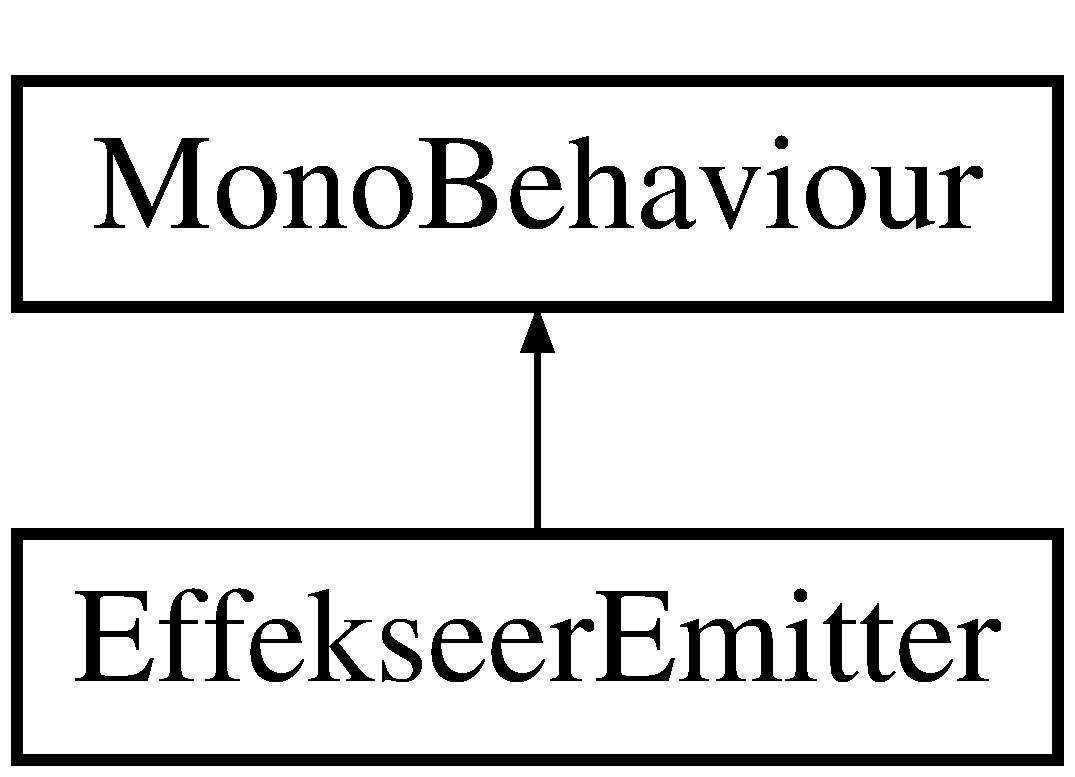
\includegraphics[height=2.000000cm]{class_effekseer_emitter}
\end{center}
\end{figure}
\subsection*{Public Member Functions}
\begin{DoxyCompactItemize}
\item 
void \hyperlink{class_effekseer_emitter_a8ae6fd4f46274d56eee5de6b1de3ee9b}{Play} (string name)
\begin{DoxyCompactList}\small\item\em エフェクトを再生 \end{DoxyCompactList}\item 
void \hyperlink{class_effekseer_emitter_a55d07e8215485e43eaa94b7b075b2f04}{Play} ()
\begin{DoxyCompactList}\small\item\em 設定されているエフェクトを再生 \end{DoxyCompactList}\item 
void \hyperlink{class_effekseer_emitter_acab7d9ae949cd0aa844ae66b2f44ad5d}{Stop} ()
\begin{DoxyCompactList}\small\item\em 再生中のエフェクトを停止 全てのエフェクトが瞬時に消える \end{DoxyCompactList}\item 
void \hyperlink{class_effekseer_emitter_a6bb4daefa3632e823b684ba575043290}{Stop\-Root} ()
\begin{DoxyCompactList}\small\item\em 再生中のエフェクトのルートノードだけを停止 ルートノードを削除したことで子ノード生成が停止され寿命で徐々に消える \end{DoxyCompactList}\item 
void \hyperlink{class_effekseer_emitter_a39366319e460cc573d4bfc40803f6787}{Set\-Target\-Location} (Vector3 target\-Location)
\begin{DoxyCompactList}\small\item\em 再生中のエフェクトのターゲット位置を設定 \end{DoxyCompactList}\end{DoxyCompactItemize}
\subsection*{Public Attributes}
\begin{DoxyCompactItemize}
\item 
string \hyperlink{class_effekseer_emitter_a3c52af81c057a2f4ea0848cb492cf208}{effect\-Name}
\begin{DoxyCompactList}\small\item\em エフェクト名 \end{DoxyCompactList}\item 
bool \hyperlink{class_effekseer_emitter_a8ff5bc48852b4a21e3b33b0cd0e8b65a}{play\-On\-Start} = false
\begin{DoxyCompactList}\small\item\em Start時に再生開始するかどうか \end{DoxyCompactList}\item 
bool \hyperlink{class_effekseer_emitter_a9b6a18e54c4b4a68bb9b81fc88b123bd}{loop} = false
\begin{DoxyCompactList}\small\item\em ループ再生するかどうか \end{DoxyCompactList}\end{DoxyCompactItemize}
\subsection*{Properties}
\begin{DoxyCompactItemize}
\item 
bool \hyperlink{class_effekseer_emitter_a5979b4e756a1f31e439752de6fb86c64}{paused}\hspace{0.3cm}{\ttfamily  \mbox{[}get, set\mbox{]}}
\begin{DoxyCompactList}\small\item\em ポーズ設定 \end{DoxyCompactList}\item 
bool \hyperlink{class_effekseer_emitter_a8beed88f3cb7357c4eb088847a6d1fbc}{shown}\hspace{0.3cm}{\ttfamily  \mbox{[}get, set\mbox{]}}
\begin{DoxyCompactList}\small\item\em 表示設定 \end{DoxyCompactList}\item 
bool \hyperlink{class_effekseer_emitter_aa4b49f6d532b7e75f2d207866ecee574}{exists}\hspace{0.3cm}{\ttfamily  \mbox{[}get\mbox{]}}
\begin{DoxyCompactList}\small\item\em 再生中のエフェクトが存在しているか \end{DoxyCompactList}\end{DoxyCompactItemize}


\subsection{Detailed Description}
エフェクトの発生源 



\subsection{Member Function Documentation}
\hypertarget{class_effekseer_emitter_a8ae6fd4f46274d56eee5de6b1de3ee9b}{\index{Effekseer\-Emitter@{Effekseer\-Emitter}!Play@{Play}}
\index{Play@{Play}!EffekseerEmitter@{Effekseer\-Emitter}}
\subsubsection[{Play}]{\setlength{\rightskip}{0pt plus 5cm}void Effekseer\-Emitter.\-Play (
\begin{DoxyParamCaption}
\item[{string}]{name}
\end{DoxyParamCaption}
)\hspace{0.3cm}{\ttfamily [inline]}}}\label{class_effekseer_emitter_a8ae6fd4f46274d56eee5de6b1de3ee9b}


エフェクトを再生 


\begin{DoxyParams}{Parameters}
{\em name} & エフェクト名\\
\hline
\end{DoxyParams}
\hypertarget{class_effekseer_emitter_a55d07e8215485e43eaa94b7b075b2f04}{\index{Effekseer\-Emitter@{Effekseer\-Emitter}!Play@{Play}}
\index{Play@{Play}!EffekseerEmitter@{Effekseer\-Emitter}}
\subsubsection[{Play}]{\setlength{\rightskip}{0pt plus 5cm}void Effekseer\-Emitter.\-Play (
\begin{DoxyParamCaption}
{}
\end{DoxyParamCaption}
)\hspace{0.3cm}{\ttfamily [inline]}}}\label{class_effekseer_emitter_a55d07e8215485e43eaa94b7b075b2f04}


設定されているエフェクトを再生 

\hypertarget{class_effekseer_emitter_a39366319e460cc573d4bfc40803f6787}{\index{Effekseer\-Emitter@{Effekseer\-Emitter}!Set\-Target\-Location@{Set\-Target\-Location}}
\index{Set\-Target\-Location@{Set\-Target\-Location}!EffekseerEmitter@{Effekseer\-Emitter}}
\subsubsection[{Set\-Target\-Location}]{\setlength{\rightskip}{0pt plus 5cm}void Effekseer\-Emitter.\-Set\-Target\-Location (
\begin{DoxyParamCaption}
\item[{Vector3}]{target\-Location}
\end{DoxyParamCaption}
)\hspace{0.3cm}{\ttfamily [inline]}}}\label{class_effekseer_emitter_a39366319e460cc573d4bfc40803f6787}


再生中のエフェクトのターゲット位置を設定 


\begin{DoxyParams}{Parameters}
{\em target\-Location} & ターゲット位置\\
\hline
\end{DoxyParams}
\hypertarget{class_effekseer_emitter_acab7d9ae949cd0aa844ae66b2f44ad5d}{\index{Effekseer\-Emitter@{Effekseer\-Emitter}!Stop@{Stop}}
\index{Stop@{Stop}!EffekseerEmitter@{Effekseer\-Emitter}}
\subsubsection[{Stop}]{\setlength{\rightskip}{0pt plus 5cm}void Effekseer\-Emitter.\-Stop (
\begin{DoxyParamCaption}
{}
\end{DoxyParamCaption}
)\hspace{0.3cm}{\ttfamily [inline]}}}\label{class_effekseer_emitter_acab7d9ae949cd0aa844ae66b2f44ad5d}


再生中のエフェクトを停止 全てのエフェクトが瞬時に消える 

\hypertarget{class_effekseer_emitter_a6bb4daefa3632e823b684ba575043290}{\index{Effekseer\-Emitter@{Effekseer\-Emitter}!Stop\-Root@{Stop\-Root}}
\index{Stop\-Root@{Stop\-Root}!EffekseerEmitter@{Effekseer\-Emitter}}
\subsubsection[{Stop\-Root}]{\setlength{\rightskip}{0pt plus 5cm}void Effekseer\-Emitter.\-Stop\-Root (
\begin{DoxyParamCaption}
{}
\end{DoxyParamCaption}
)\hspace{0.3cm}{\ttfamily [inline]}}}\label{class_effekseer_emitter_a6bb4daefa3632e823b684ba575043290}


再生中のエフェクトのルートノードだけを停止 ルートノードを削除したことで子ノード生成が停止され寿命で徐々に消える 



\subsection{Member Data Documentation}
\hypertarget{class_effekseer_emitter_a3c52af81c057a2f4ea0848cb492cf208}{\index{Effekseer\-Emitter@{Effekseer\-Emitter}!effect\-Name@{effect\-Name}}
\index{effect\-Name@{effect\-Name}!EffekseerEmitter@{Effekseer\-Emitter}}
\subsubsection[{effect\-Name}]{\setlength{\rightskip}{0pt plus 5cm}string Effekseer\-Emitter.\-effect\-Name}}\label{class_effekseer_emitter_a3c52af81c057a2f4ea0848cb492cf208}


エフェクト名 

\hypertarget{class_effekseer_emitter_a9b6a18e54c4b4a68bb9b81fc88b123bd}{\index{Effekseer\-Emitter@{Effekseer\-Emitter}!loop@{loop}}
\index{loop@{loop}!EffekseerEmitter@{Effekseer\-Emitter}}
\subsubsection[{loop}]{\setlength{\rightskip}{0pt plus 5cm}bool Effekseer\-Emitter.\-loop = false}}\label{class_effekseer_emitter_a9b6a18e54c4b4a68bb9b81fc88b123bd}


ループ再生するかどうか 

\hypertarget{class_effekseer_emitter_a8ff5bc48852b4a21e3b33b0cd0e8b65a}{\index{Effekseer\-Emitter@{Effekseer\-Emitter}!play\-On\-Start@{play\-On\-Start}}
\index{play\-On\-Start@{play\-On\-Start}!EffekseerEmitter@{Effekseer\-Emitter}}
\subsubsection[{play\-On\-Start}]{\setlength{\rightskip}{0pt plus 5cm}bool Effekseer\-Emitter.\-play\-On\-Start = false}}\label{class_effekseer_emitter_a8ff5bc48852b4a21e3b33b0cd0e8b65a}


Start時に再生開始するかどうか 



\subsection{Property Documentation}
\hypertarget{class_effekseer_emitter_aa4b49f6d532b7e75f2d207866ecee574}{\index{Effekseer\-Emitter@{Effekseer\-Emitter}!exists@{exists}}
\index{exists@{exists}!EffekseerEmitter@{Effekseer\-Emitter}}
\subsubsection[{exists}]{\setlength{\rightskip}{0pt plus 5cm}bool Effekseer\-Emitter.\-exists\hspace{0.3cm}{\ttfamily [get]}}}\label{class_effekseer_emitter_aa4b49f6d532b7e75f2d207866ecee574}


再生中のエフェクトが存在しているか 

true\-: 存在している

false\-: 再生終了で破棄。もしくは\-Stopで停止された\hypertarget{class_effekseer_emitter_a5979b4e756a1f31e439752de6fb86c64}{\index{Effekseer\-Emitter@{Effekseer\-Emitter}!paused@{paused}}
\index{paused@{paused}!EffekseerEmitter@{Effekseer\-Emitter}}
\subsubsection[{paused}]{\setlength{\rightskip}{0pt plus 5cm}bool Effekseer\-Emitter.\-paused\hspace{0.3cm}{\ttfamily [get]}, {\ttfamily [set]}}}\label{class_effekseer_emitter_a5979b4e756a1f31e439752de6fb86c64}


ポーズ設定 

true\-: 停止中。\-Updateで更新しない

false\-: 再生中。\-Updateで更新する\hypertarget{class_effekseer_emitter_a8beed88f3cb7357c4eb088847a6d1fbc}{\index{Effekseer\-Emitter@{Effekseer\-Emitter}!shown@{shown}}
\index{shown@{shown}!EffekseerEmitter@{Effekseer\-Emitter}}
\subsubsection[{shown}]{\setlength{\rightskip}{0pt plus 5cm}bool Effekseer\-Emitter.\-shown\hspace{0.3cm}{\ttfamily [get]}, {\ttfamily [set]}}}\label{class_effekseer_emitter_a8beed88f3cb7357c4eb088847a6d1fbc}


表示設定 

true\-: 表示\-O\-N。\-Drawで描画する

false\-: 表示\-O\-F\-F。\-Drawで描画しない

The documentation for this class was generated from the following file\-:\begin{DoxyCompactItemize}
\item 
dev/\-Cpp/\-Unity\-Plugin/\-Unity\-Script/Effekseer\-Emitter.\-cs\end{DoxyCompactItemize}

\hypertarget{struct_effekseer_handle}{\section{Effekseer\-Handle Struct Reference}
\label{struct_effekseer_handle}\index{Effekseer\-Handle@{Effekseer\-Handle}}
}


再生したエフェクトのインスタンスハンドル  


\subsection*{Public Member Functions}
\begin{DoxyCompactItemize}
\item 
\hypertarget{struct_effekseer_handle_a396167b208bb830dd0fcd65d677d0ab9}{{\bfseries Effekseer\-Handle} (int handle)}\label{struct_effekseer_handle_a396167b208bb830dd0fcd65d677d0ab9}

\item 
void \hyperlink{struct_effekseer_handle_add31723e9d75fad60015c48dfe1bf785}{Stop} ()
\begin{DoxyCompactList}\small\item\em エフェクトを停止する 全てのエフェクトが瞬時に消える \end{DoxyCompactList}\item 
void \hyperlink{struct_effekseer_handle_ae16184a6f1770d63edf941941b8ad063}{Stop\-Root} ()
\begin{DoxyCompactList}\small\item\em 再生中のエフェクトのルートノードだけを停止 ルートノードを削除したことで子ノード生成が停止され寿命で徐々に消える \end{DoxyCompactList}\item 
void \hyperlink{struct_effekseer_handle_a65d631a161e475acac133b6db28d0070}{Set\-Location} (Vector3 location)
\begin{DoxyCompactList}\small\item\em エフェクトの位置を設定 \end{DoxyCompactList}\item 
void \hyperlink{struct_effekseer_handle_a54be425dc9d059e66fe00799f34e25cf}{Set\-Rotation} (Quaternion rotation)
\begin{DoxyCompactList}\small\item\em エフェクトの回転を設定 \end{DoxyCompactList}\item 
void \hyperlink{struct_effekseer_handle_a858d40ff7676ec5c2ae062596f52795b}{Set\-Scale} (Vector3 scale)
\begin{DoxyCompactList}\small\item\em エフェクトの拡縮を設定 \end{DoxyCompactList}\item 
void \hyperlink{struct_effekseer_handle_aa13ed72d63bdcf16ab9683261b92c855}{Set\-Target\-Location} (Vector3 target\-Location)
\begin{DoxyCompactList}\small\item\em エフェクトのターゲット位置を設定 \end{DoxyCompactList}\end{DoxyCompactItemize}
\subsection*{Properties}
\begin{DoxyCompactItemize}
\item 
bool \hyperlink{struct_effekseer_handle_a3ba9bf72308429369214fd10ebb86ca6}{paused}\hspace{0.3cm}{\ttfamily  \mbox{[}get, set\mbox{]}}
\begin{DoxyCompactList}\small\item\em ポーズ設定 \end{DoxyCompactList}\item 
bool \hyperlink{struct_effekseer_handle_a96d0ebfe4cab721aaea0992b1750ae43}{shown}\hspace{0.3cm}{\ttfamily  \mbox{[}get, set\mbox{]}}
\begin{DoxyCompactList}\small\item\em 表示設定 \end{DoxyCompactList}\item 
bool \hyperlink{struct_effekseer_handle_a2eabd884f8b23833cbf69f3f9d9c875b}{enable}\hspace{0.3cm}{\ttfamily  \mbox{[}get\mbox{]}}
\begin{DoxyCompactList}\small\item\em インスタンスハンドルが有効かどうか\par
 \end{DoxyCompactList}\item 
bool \hyperlink{struct_effekseer_handle_ac1d253853e6471ce1e3c951491803c27}{exists}\hspace{0.3cm}{\ttfamily  \mbox{[}get\mbox{]}}
\begin{DoxyCompactList}\small\item\em エフェクトのインスタンスが存在しているかどうか \end{DoxyCompactList}\end{DoxyCompactItemize}


\subsection{Detailed Description}
再生したエフェクトのインスタンスハンドル 



\subsection{Member Function Documentation}
\hypertarget{struct_effekseer_handle_a65d631a161e475acac133b6db28d0070}{\index{Effekseer\-Handle@{Effekseer\-Handle}!Set\-Location@{Set\-Location}}
\index{Set\-Location@{Set\-Location}!EffekseerHandle@{Effekseer\-Handle}}
\subsubsection[{Set\-Location}]{\setlength{\rightskip}{0pt plus 5cm}void Effekseer\-Handle.\-Set\-Location (
\begin{DoxyParamCaption}
\item[{Vector3}]{location}
\end{DoxyParamCaption}
)\hspace{0.3cm}{\ttfamily [inline]}}}\label{struct_effekseer_handle_a65d631a161e475acac133b6db28d0070}


エフェクトの位置を設定 


\begin{DoxyParams}{Parameters}
{\em location} & 位置\\
\hline
\end{DoxyParams}
\hypertarget{struct_effekseer_handle_a54be425dc9d059e66fe00799f34e25cf}{\index{Effekseer\-Handle@{Effekseer\-Handle}!Set\-Rotation@{Set\-Rotation}}
\index{Set\-Rotation@{Set\-Rotation}!EffekseerHandle@{Effekseer\-Handle}}
\subsubsection[{Set\-Rotation}]{\setlength{\rightskip}{0pt plus 5cm}void Effekseer\-Handle.\-Set\-Rotation (
\begin{DoxyParamCaption}
\item[{Quaternion}]{rotation}
\end{DoxyParamCaption}
)\hspace{0.3cm}{\ttfamily [inline]}}}\label{struct_effekseer_handle_a54be425dc9d059e66fe00799f34e25cf}


エフェクトの回転を設定 


\begin{DoxyParams}{Parameters}
{\em rotation} & 回転\\
\hline
\end{DoxyParams}
\hypertarget{struct_effekseer_handle_a858d40ff7676ec5c2ae062596f52795b}{\index{Effekseer\-Handle@{Effekseer\-Handle}!Set\-Scale@{Set\-Scale}}
\index{Set\-Scale@{Set\-Scale}!EffekseerHandle@{Effekseer\-Handle}}
\subsubsection[{Set\-Scale}]{\setlength{\rightskip}{0pt plus 5cm}void Effekseer\-Handle.\-Set\-Scale (
\begin{DoxyParamCaption}
\item[{Vector3}]{scale}
\end{DoxyParamCaption}
)\hspace{0.3cm}{\ttfamily [inline]}}}\label{struct_effekseer_handle_a858d40ff7676ec5c2ae062596f52795b}


エフェクトの拡縮を設定 


\begin{DoxyParams}{Parameters}
{\em scale} & 拡縮\\
\hline
\end{DoxyParams}
\hypertarget{struct_effekseer_handle_aa13ed72d63bdcf16ab9683261b92c855}{\index{Effekseer\-Handle@{Effekseer\-Handle}!Set\-Target\-Location@{Set\-Target\-Location}}
\index{Set\-Target\-Location@{Set\-Target\-Location}!EffekseerHandle@{Effekseer\-Handle}}
\subsubsection[{Set\-Target\-Location}]{\setlength{\rightskip}{0pt plus 5cm}void Effekseer\-Handle.\-Set\-Target\-Location (
\begin{DoxyParamCaption}
\item[{Vector3}]{target\-Location}
\end{DoxyParamCaption}
)\hspace{0.3cm}{\ttfamily [inline]}}}\label{struct_effekseer_handle_aa13ed72d63bdcf16ab9683261b92c855}


エフェクトのターゲット位置を設定 


\begin{DoxyParams}{Parameters}
{\em target\-Location} & ターゲット位置\\
\hline
\end{DoxyParams}
\hypertarget{struct_effekseer_handle_add31723e9d75fad60015c48dfe1bf785}{\index{Effekseer\-Handle@{Effekseer\-Handle}!Stop@{Stop}}
\index{Stop@{Stop}!EffekseerHandle@{Effekseer\-Handle}}
\subsubsection[{Stop}]{\setlength{\rightskip}{0pt plus 5cm}void Effekseer\-Handle.\-Stop (
\begin{DoxyParamCaption}
{}
\end{DoxyParamCaption}
)\hspace{0.3cm}{\ttfamily [inline]}}}\label{struct_effekseer_handle_add31723e9d75fad60015c48dfe1bf785}


エフェクトを停止する 全てのエフェクトが瞬時に消える 

\hypertarget{struct_effekseer_handle_ae16184a6f1770d63edf941941b8ad063}{\index{Effekseer\-Handle@{Effekseer\-Handle}!Stop\-Root@{Stop\-Root}}
\index{Stop\-Root@{Stop\-Root}!EffekseerHandle@{Effekseer\-Handle}}
\subsubsection[{Stop\-Root}]{\setlength{\rightskip}{0pt plus 5cm}void Effekseer\-Handle.\-Stop\-Root (
\begin{DoxyParamCaption}
{}
\end{DoxyParamCaption}
)\hspace{0.3cm}{\ttfamily [inline]}}}\label{struct_effekseer_handle_ae16184a6f1770d63edf941941b8ad063}


再生中のエフェクトのルートノードだけを停止 ルートノードを削除したことで子ノード生成が停止され寿命で徐々に消える 



\subsection{Property Documentation}
\hypertarget{struct_effekseer_handle_a2eabd884f8b23833cbf69f3f9d9c875b}{\index{Effekseer\-Handle@{Effekseer\-Handle}!enable@{enable}}
\index{enable@{enable}!EffekseerHandle@{Effekseer\-Handle}}
\subsubsection[{enable}]{\setlength{\rightskip}{0pt plus 5cm}bool Effekseer\-Handle.\-enable\hspace{0.3cm}{\ttfamily [get]}}}\label{struct_effekseer_handle_a2eabd884f8b23833cbf69f3f9d9c875b}


インスタンスハンドルが有効かどうか\par
 

true\-: 有効

false\-: 無効\hypertarget{struct_effekseer_handle_ac1d253853e6471ce1e3c951491803c27}{\index{Effekseer\-Handle@{Effekseer\-Handle}!exists@{exists}}
\index{exists@{exists}!EffekseerHandle@{Effekseer\-Handle}}
\subsubsection[{exists}]{\setlength{\rightskip}{0pt plus 5cm}bool Effekseer\-Handle.\-exists\hspace{0.3cm}{\ttfamily [get]}}}\label{struct_effekseer_handle_ac1d253853e6471ce1e3c951491803c27}


エフェクトのインスタンスが存在しているかどうか 

true\-: 存在している

false\-: 再生終了で破棄。もしくは\-Stopで停止された\hypertarget{struct_effekseer_handle_a3ba9bf72308429369214fd10ebb86ca6}{\index{Effekseer\-Handle@{Effekseer\-Handle}!paused@{paused}}
\index{paused@{paused}!EffekseerHandle@{Effekseer\-Handle}}
\subsubsection[{paused}]{\setlength{\rightskip}{0pt plus 5cm}bool Effekseer\-Handle.\-paused\hspace{0.3cm}{\ttfamily [get]}, {\ttfamily [set]}}}\label{struct_effekseer_handle_a3ba9bf72308429369214fd10ebb86ca6}


ポーズ設定 

true\-: 停止中。\-Updateで更新しない

false\-: 再生中。\-Updateで更新する\hypertarget{struct_effekseer_handle_a96d0ebfe4cab721aaea0992b1750ae43}{\index{Effekseer\-Handle@{Effekseer\-Handle}!shown@{shown}}
\index{shown@{shown}!EffekseerHandle@{Effekseer\-Handle}}
\subsubsection[{shown}]{\setlength{\rightskip}{0pt plus 5cm}bool Effekseer\-Handle.\-shown\hspace{0.3cm}{\ttfamily [get]}, {\ttfamily [set]}}}\label{struct_effekseer_handle_a96d0ebfe4cab721aaea0992b1750ae43}


表示設定 

true\-: 表示\-O\-N。\-Drawで描画する

false\-: 表示\-O\-F\-F。\-Drawで描画しない

The documentation for this struct was generated from the following file\-:\begin{DoxyCompactItemize}
\item 
dev/\-Cpp/\-Unity\-Plugin/\-Unity\-Script/Effekseer\-System.\-cs\end{DoxyCompactItemize}

\hypertarget{class_effekseer_system}{\section{Effekseer\-System Class Reference}
\label{class_effekseer_system}\index{Effekseer\-System@{Effekseer\-System}}
}
Inheritance diagram for Effekseer\-System\-:\begin{figure}[H]
\begin{center}
\leavevmode
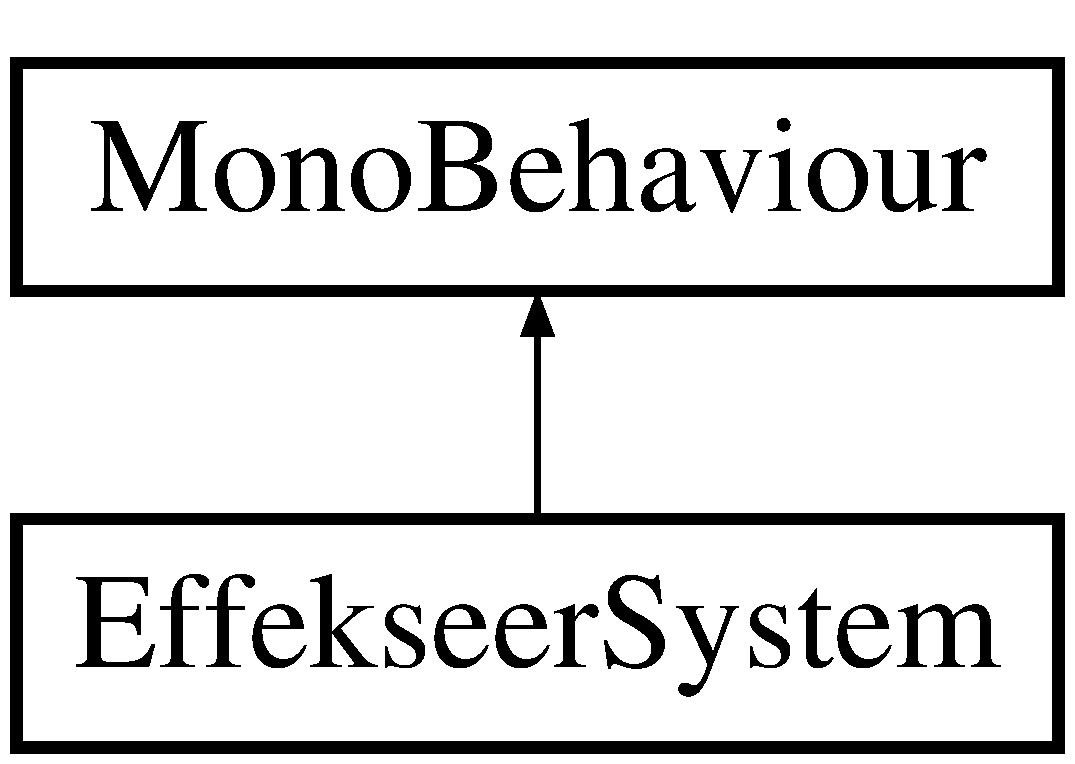
\includegraphics[height=2.000000cm]{class_effekseer_system}
\end{center}
\end{figure}
\subsection*{Static Public Member Functions}
\begin{DoxyCompactItemize}
\item 
static \hyperlink{struct_effekseer_handle}{Effekseer\-Handle} \hyperlink{class_effekseer_system_a8d0a7561a512b64acce39c4456ff6f37}{Play\-Effect} (string name, Vector3 location)
\begin{DoxyCompactList}\small\item\em エフェクトの再生 \end{DoxyCompactList}\item 
static void \hyperlink{class_effekseer_system_acf3dde4a65c0e99aeacfea71b517b541}{Stop\-All\-Effects} ()
\begin{DoxyCompactList}\small\item\em 全エフェクトの再生停止 \end{DoxyCompactList}\item 
static void \hyperlink{class_effekseer_system_af4059b796725905982565d8b239bf9fa}{Load\-Effect} (string name)
\begin{DoxyCompactList}\small\item\em エフェクトのロード(Resourcesから) \end{DoxyCompactList}\item 
static void \hyperlink{class_effekseer_system_a4f7d874f76c4f354b70b852df590be72}{Load\-Effect} (string name, Asset\-Bundle asset\-Bundle)
\begin{DoxyCompactList}\small\item\em エフェクトのロード(Asset\-Bundleから) \end{DoxyCompactList}\item 
static void \hyperlink{class_effekseer_system_a8b328c83692b922217657a21f9d5fdeb}{Release\-Effect} (string name)
\begin{DoxyCompactList}\small\item\em エフェクトの解放 \end{DoxyCompactList}\end{DoxyCompactItemize}
\subsection*{Public Attributes}
\begin{DoxyCompactItemize}
\item 
bool \hyperlink{class_effekseer_system_a469cf59d9deeaef6e27b15c5fc5ee524}{draw\-In\-Scene\-View} = true
\begin{DoxyCompactList}\small\item\em シーンビューに描画するかどうか \end{DoxyCompactList}\item 
int \hyperlink{class_effekseer_system_a0516609db2194d83016f439b93510f21}{effect\-Instances} = 800
\begin{DoxyCompactList}\small\item\em エフェクトインスタンスの最大数 \end{DoxyCompactList}\item 
int \hyperlink{class_effekseer_system_a2007e297eab6bc504cce40650679b1c4}{max\-Squares} = 1200
\begin{DoxyCompactList}\small\item\em 描画できる四角形の最大数 \end{DoxyCompactList}\item 
int \hyperlink{class_effekseer_system_ac83155c54d94fc6b61f6f53032923667}{sound\-Instances} = 16
\begin{DoxyCompactList}\small\item\em サウンドインスタンスの最大数 \end{DoxyCompactList}\end{DoxyCompactItemize}
\subsection*{Properties}
\begin{DoxyCompactItemize}
\item 
\hypertarget{class_effekseer_system_abaa89ed68be2a0ff10f1ab7b04ce219a}{static \hyperlink{class_effekseer_system}{Effekseer\-System} {\bfseries Instance}\hspace{0.3cm}{\ttfamily  \mbox{[}get\mbox{]}}}\label{class_effekseer_system_abaa89ed68be2a0ff10f1ab7b04ce219a}

\end{DoxyCompactItemize}


\subsection{Member Function Documentation}
\hypertarget{class_effekseer_system_af4059b796725905982565d8b239bf9fa}{\index{Effekseer\-System@{Effekseer\-System}!Load\-Effect@{Load\-Effect}}
\index{Load\-Effect@{Load\-Effect}!EffekseerSystem@{Effekseer\-System}}
\subsubsection[{Load\-Effect}]{\setlength{\rightskip}{0pt plus 5cm}static void Effekseer\-System.\-Load\-Effect (
\begin{DoxyParamCaption}
\item[{string}]{name}
\end{DoxyParamCaption}
)\hspace{0.3cm}{\ttfamily [inline]}, {\ttfamily [static]}}}\label{class_effekseer_system_af4059b796725905982565d8b239bf9fa}


エフェクトのロード(Resourcesから) 


\begin{DoxyParams}{Parameters}
{\em name} & エフェクト名(efkファイルの名前から\char`\"{}.\-efk\char`\"{}を取り除いたもの)\\
\hline
\end{DoxyParams}
\hypertarget{class_effekseer_system_a4f7d874f76c4f354b70b852df590be72}{\index{Effekseer\-System@{Effekseer\-System}!Load\-Effect@{Load\-Effect}}
\index{Load\-Effect@{Load\-Effect}!EffekseerSystem@{Effekseer\-System}}
\subsubsection[{Load\-Effect}]{\setlength{\rightskip}{0pt plus 5cm}static void Effekseer\-System.\-Load\-Effect (
\begin{DoxyParamCaption}
\item[{string}]{name, }
\item[{Asset\-Bundle}]{asset\-Bundle}
\end{DoxyParamCaption}
)\hspace{0.3cm}{\ttfamily [inline]}, {\ttfamily [static]}}}\label{class_effekseer_system_a4f7d874f76c4f354b70b852df590be72}


エフェクトのロード(Asset\-Bundleから) 


\begin{DoxyParams}{Parameters}
{\em name} & エフェクト名(efkファイルの名前から\char`\"{}.\-efk\char`\"{}を取り除いたもの)\\
\hline
\end{DoxyParams}
\hypertarget{class_effekseer_system_a8d0a7561a512b64acce39c4456ff6f37}{\index{Effekseer\-System@{Effekseer\-System}!Play\-Effect@{Play\-Effect}}
\index{Play\-Effect@{Play\-Effect}!EffekseerSystem@{Effekseer\-System}}
\subsubsection[{Play\-Effect}]{\setlength{\rightskip}{0pt plus 5cm}static {\bf Effekseer\-Handle} Effekseer\-System.\-Play\-Effect (
\begin{DoxyParamCaption}
\item[{string}]{name, }
\item[{Vector3}]{location}
\end{DoxyParamCaption}
)\hspace{0.3cm}{\ttfamily [inline]}, {\ttfamily [static]}}}\label{class_effekseer_system_a8d0a7561a512b64acce39c4456ff6f37}


エフェクトの再生 


\begin{DoxyParams}{Parameters}
{\em name} & エフェクト名\\
\hline
{\em location} & 再生開始する位置\\
\hline
\end{DoxyParams}
\begin{DoxyReturn}{Returns}
再生したエフェクトのハンドル
\end{DoxyReturn}
\hypertarget{class_effekseer_system_a8b328c83692b922217657a21f9d5fdeb}{\index{Effekseer\-System@{Effekseer\-System}!Release\-Effect@{Release\-Effect}}
\index{Release\-Effect@{Release\-Effect}!EffekseerSystem@{Effekseer\-System}}
\subsubsection[{Release\-Effect}]{\setlength{\rightskip}{0pt plus 5cm}static void Effekseer\-System.\-Release\-Effect (
\begin{DoxyParamCaption}
\item[{string}]{name}
\end{DoxyParamCaption}
)\hspace{0.3cm}{\ttfamily [inline]}, {\ttfamily [static]}}}\label{class_effekseer_system_a8b328c83692b922217657a21f9d5fdeb}


エフェクトの解放 


\begin{DoxyParams}{Parameters}
{\em name} & エフェクト名(efkファイルの名前から\char`\"{}.\-efk\char`\"{}を取り除いたもの)\\
\hline
\end{DoxyParams}
\hypertarget{class_effekseer_system_acf3dde4a65c0e99aeacfea71b517b541}{\index{Effekseer\-System@{Effekseer\-System}!Stop\-All\-Effects@{Stop\-All\-Effects}}
\index{Stop\-All\-Effects@{Stop\-All\-Effects}!EffekseerSystem@{Effekseer\-System}}
\subsubsection[{Stop\-All\-Effects}]{\setlength{\rightskip}{0pt plus 5cm}static void Effekseer\-System.\-Stop\-All\-Effects (
\begin{DoxyParamCaption}
{}
\end{DoxyParamCaption}
)\hspace{0.3cm}{\ttfamily [inline]}, {\ttfamily [static]}}}\label{class_effekseer_system_acf3dde4a65c0e99aeacfea71b517b541}


全エフェクトの再生停止 



\subsection{Member Data Documentation}
\hypertarget{class_effekseer_system_a469cf59d9deeaef6e27b15c5fc5ee524}{\index{Effekseer\-System@{Effekseer\-System}!draw\-In\-Scene\-View@{draw\-In\-Scene\-View}}
\index{draw\-In\-Scene\-View@{draw\-In\-Scene\-View}!EffekseerSystem@{Effekseer\-System}}
\subsubsection[{draw\-In\-Scene\-View}]{\setlength{\rightskip}{0pt plus 5cm}bool Effekseer\-System.\-draw\-In\-Scene\-View = true}}\label{class_effekseer_system_a469cf59d9deeaef6e27b15c5fc5ee524}


シーンビューに描画するかどうか 

\hypertarget{class_effekseer_system_a0516609db2194d83016f439b93510f21}{\index{Effekseer\-System@{Effekseer\-System}!effect\-Instances@{effect\-Instances}}
\index{effect\-Instances@{effect\-Instances}!EffekseerSystem@{Effekseer\-System}}
\subsubsection[{effect\-Instances}]{\setlength{\rightskip}{0pt plus 5cm}int Effekseer\-System.\-effect\-Instances = 800}}\label{class_effekseer_system_a0516609db2194d83016f439b93510f21}


エフェクトインスタンスの最大数 

\hypertarget{class_effekseer_system_a2007e297eab6bc504cce40650679b1c4}{\index{Effekseer\-System@{Effekseer\-System}!max\-Squares@{max\-Squares}}
\index{max\-Squares@{max\-Squares}!EffekseerSystem@{Effekseer\-System}}
\subsubsection[{max\-Squares}]{\setlength{\rightskip}{0pt plus 5cm}int Effekseer\-System.\-max\-Squares = 1200}}\label{class_effekseer_system_a2007e297eab6bc504cce40650679b1c4}


描画できる四角形の最大数 

\hypertarget{class_effekseer_system_ac83155c54d94fc6b61f6f53032923667}{\index{Effekseer\-System@{Effekseer\-System}!sound\-Instances@{sound\-Instances}}
\index{sound\-Instances@{sound\-Instances}!EffekseerSystem@{Effekseer\-System}}
\subsubsection[{sound\-Instances}]{\setlength{\rightskip}{0pt plus 5cm}int Effekseer\-System.\-sound\-Instances = 16}}\label{class_effekseer_system_ac83155c54d94fc6b61f6f53032923667}


サウンドインスタンスの最大数 



The documentation for this class was generated from the following file\-:\begin{DoxyCompactItemize}
\item 
dev/\-Cpp/\-Unity\-Plugin/\-Unity\-Script/Effekseer\-System.\-cs\end{DoxyCompactItemize}

\hypertarget{class_effekseer_1_1_sound_instance}{\section{Effekseer.\-Sound\-Instance Class Reference}
\label{class_effekseer_1_1_sound_instance}\index{Effekseer.\-Sound\-Instance@{Effekseer.\-Sound\-Instance}}
}
Inheritance diagram for Effekseer.\-Sound\-Instance\-:\begin{figure}[H]
\begin{center}
\leavevmode
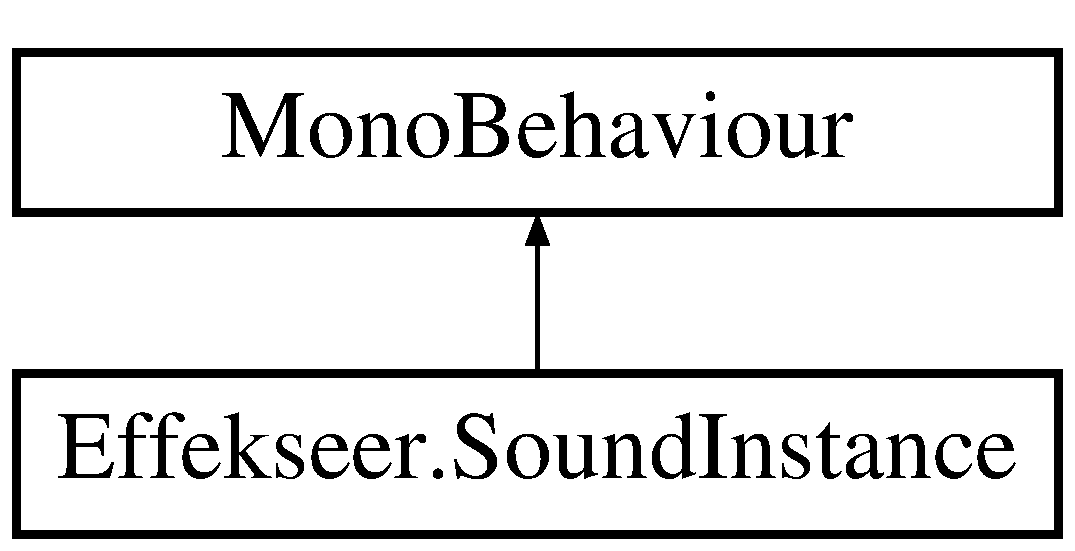
\includegraphics[height=2.000000cm]{class_effekseer_1_1_sound_instance}
\end{center}
\end{figure}
\subsection*{Public Member Functions}
\begin{DoxyCompactItemize}
\item 
\hypertarget{class_effekseer_1_1_sound_instance_a0dad13c99eec9f7fd3a254da889d41b0}{void {\bfseries Play} (string tag, Audio\-Clip clip, float volume, float pan, float pitch, bool mode3\-D, float x, float y, float z, float distance)}\label{class_effekseer_1_1_sound_instance_a0dad13c99eec9f7fd3a254da889d41b0}

\item 
\hypertarget{class_effekseer_1_1_sound_instance_a47120b96077ba0222ba7dcaac289947f}{void {\bfseries Stop} ()}\label{class_effekseer_1_1_sound_instance_a47120b96077ba0222ba7dcaac289947f}

\item 
\hypertarget{class_effekseer_1_1_sound_instance_a8bea651d2b06d9f9cf4cefc97a9f7226}{void {\bfseries Pause} (bool paused)}\label{class_effekseer_1_1_sound_instance_a8bea651d2b06d9f9cf4cefc97a9f7226}

\item 
\hypertarget{class_effekseer_1_1_sound_instance_aba66c6f052a23feff462c6ceebd09b2e}{bool {\bfseries Check\-Playing} ()}\label{class_effekseer_1_1_sound_instance_aba66c6f052a23feff462c6ceebd09b2e}

\end{DoxyCompactItemize}
\subsection*{Public Attributes}
\begin{DoxyCompactItemize}
\item 
\hypertarget{class_effekseer_1_1_sound_instance_aaecb9b470d568fa58a7b89d9b8374e65}{string {\bfseries Audio\-Tag}}\label{class_effekseer_1_1_sound_instance_aaecb9b470d568fa58a7b89d9b8374e65}

\end{DoxyCompactItemize}


The documentation for this class was generated from the following file\-:\begin{DoxyCompactItemize}
\item 
dev/\-Cpp/\-Unity\-Plugin/\-Unity\-Script/Effekseer.\-cs\end{DoxyCompactItemize}

%--- End generated contents ---

% Index
\newpage
\phantomsection
\addcontentsline{toc}{part}{Index}
\printindex

\end{document}
